\chapter{Audio compressive sensing}
\label{chap:audio-cs}
In this chapter, I apply CS to audio signals. These type of signals act as the bridge to $N$-dimensional CS as they are one-dimensional when represented in the time domain, but are projected to higher dimensions when represented in another domain, such as the spectrogram/modulation domain. Unlike images, audio signals are a tad harder to compressively sample. Due to their relatively higher information density, the effects of undersampling are easily observed.

\section{Test case: Sinusoid redux}
\label{sec:audio-sine}
In this test case, I recorded a guitar playing a single E$_4$ (330 Hz) note at the standard 44.1 kHz sampling rate for 4 seconds. Since the Nyquist rate of the actual signal is 660 Hz, the recording can be downsampled to a practical 8 kHz for processing. The signal waveform and frequency content is shown in Fig.~\ref{fig:guitar-original}. The base frequency is dominant in the frequency spectrum, and several harmonics can be observed. The goal here is to be able to recover the harmonics that have a frequency higher than the compressive sampling rate.

The compressed signal is shown in Fig.~\ref{fig:guitar-compressed}, which was compressively sampled with a quasi-frequency of 1000~Hz (1000 i.i.d.~random samples per second), corresponding to a 12.5\% compression ratio. The waveform envelope still resembles that of the original, but due to the random nature of sampling, the periodicity is not preserved, and is reflected in the seemingly random frequency content.

Following a similar process shown in Chapter \ref{chap:random-cs}, I chose DCT to be the sparse representation domain, and LASSO as the optimization algorithm. The reconstructed signal is shown in Fig.~\ref{fig:guitar-recovered}.For this case, I am concerned only with the frequency components that are recovered, and not so much with the magnitude. Thus, the reconstruction quality can be quantified using the cosine similarity

\begin{equation}
	\label{eq:cossim}
	\mathrm{similarity} = \cos\theta = \frac{\vec{x} \cdot \bm\hat{\vec{x}}}{\norm{\vec{x}}_2 \norm{\bm\hat{\vec{x}}}_2}
\end{equation}

\noindent which allows us to compare two signals' frequency content directly in the time domain. A cosine similarity value of 0.8 and above indicates acceptable quality; a value of 1.0 indicates perfect reconstruction.

\begin{figure}[htb]
	\centering
	\begin{subfigure}{\textwidth}
		\centering
		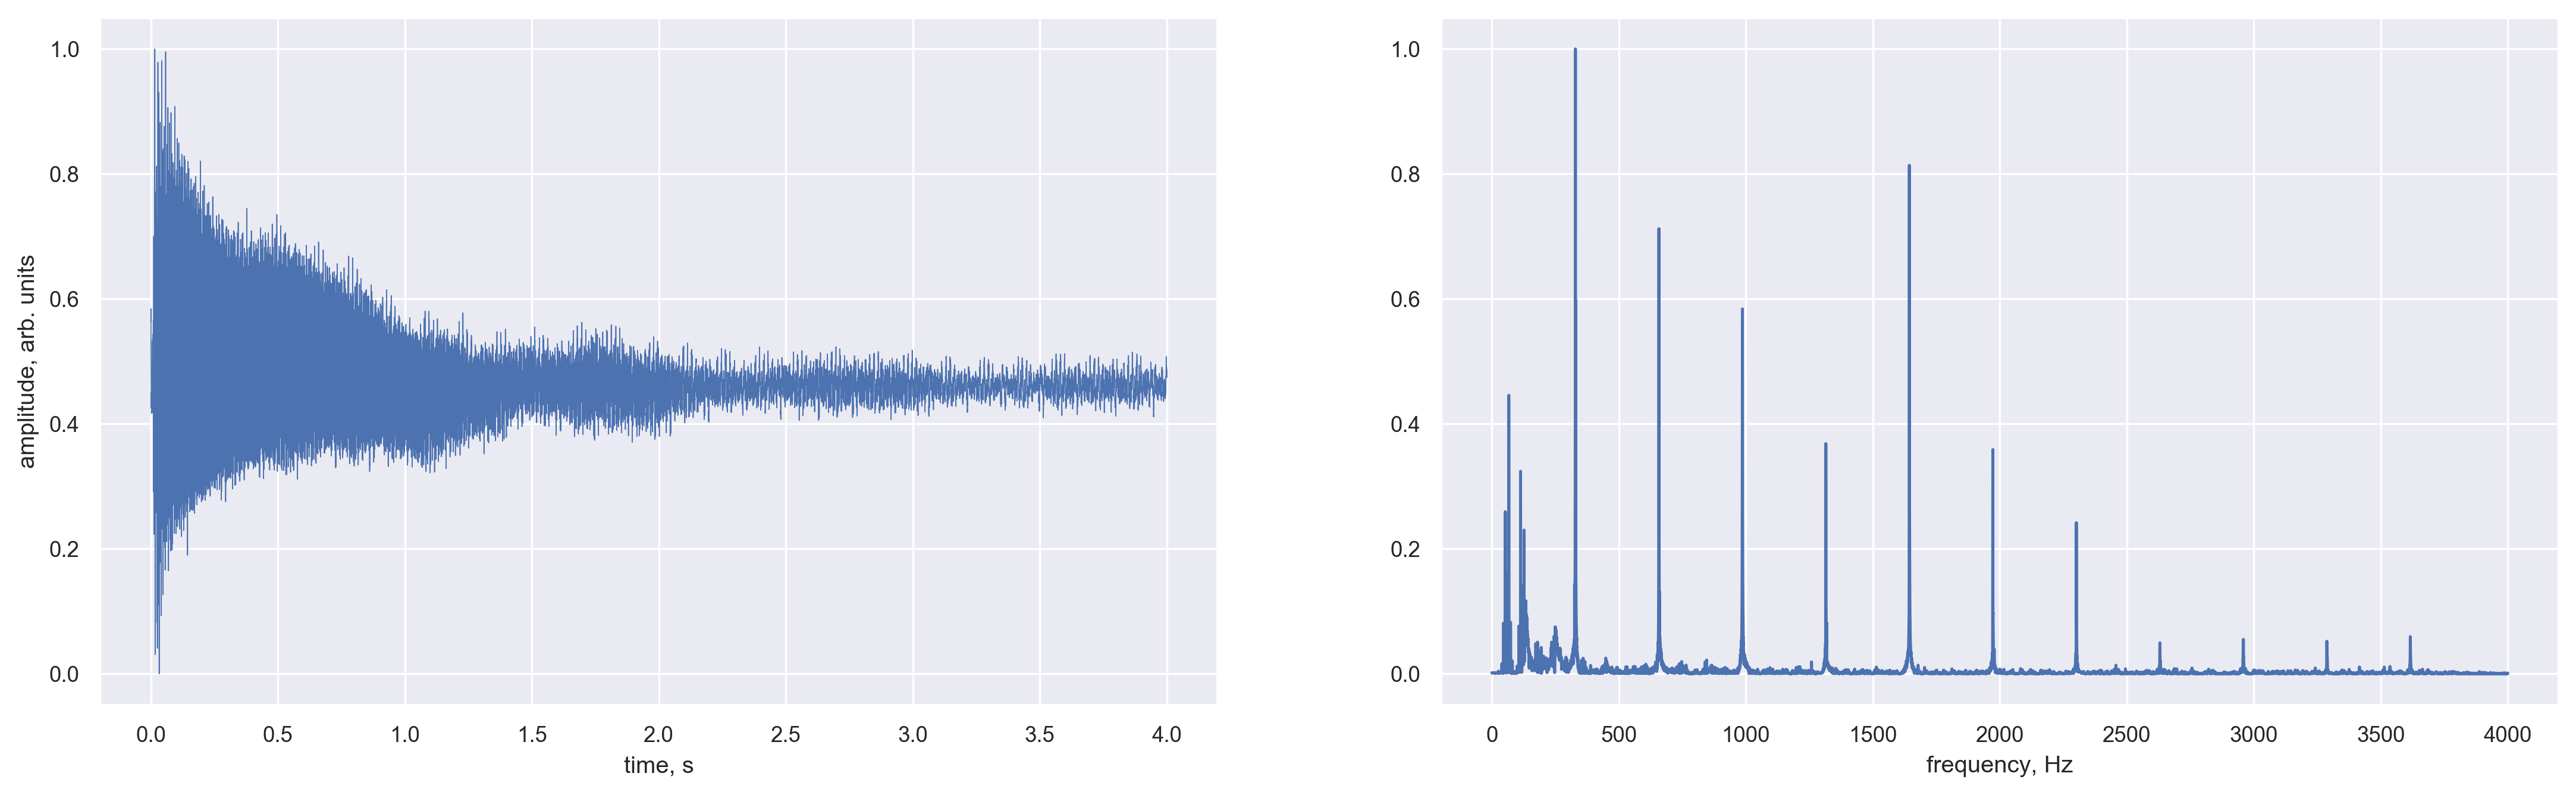
\includegraphics[width=\textwidth]{E1_orig.png}
		\caption{Original}
		\label{fig:guitar-original}
	\end{subfigure}
	\begin{subfigure}{\textwidth}
		\centering
		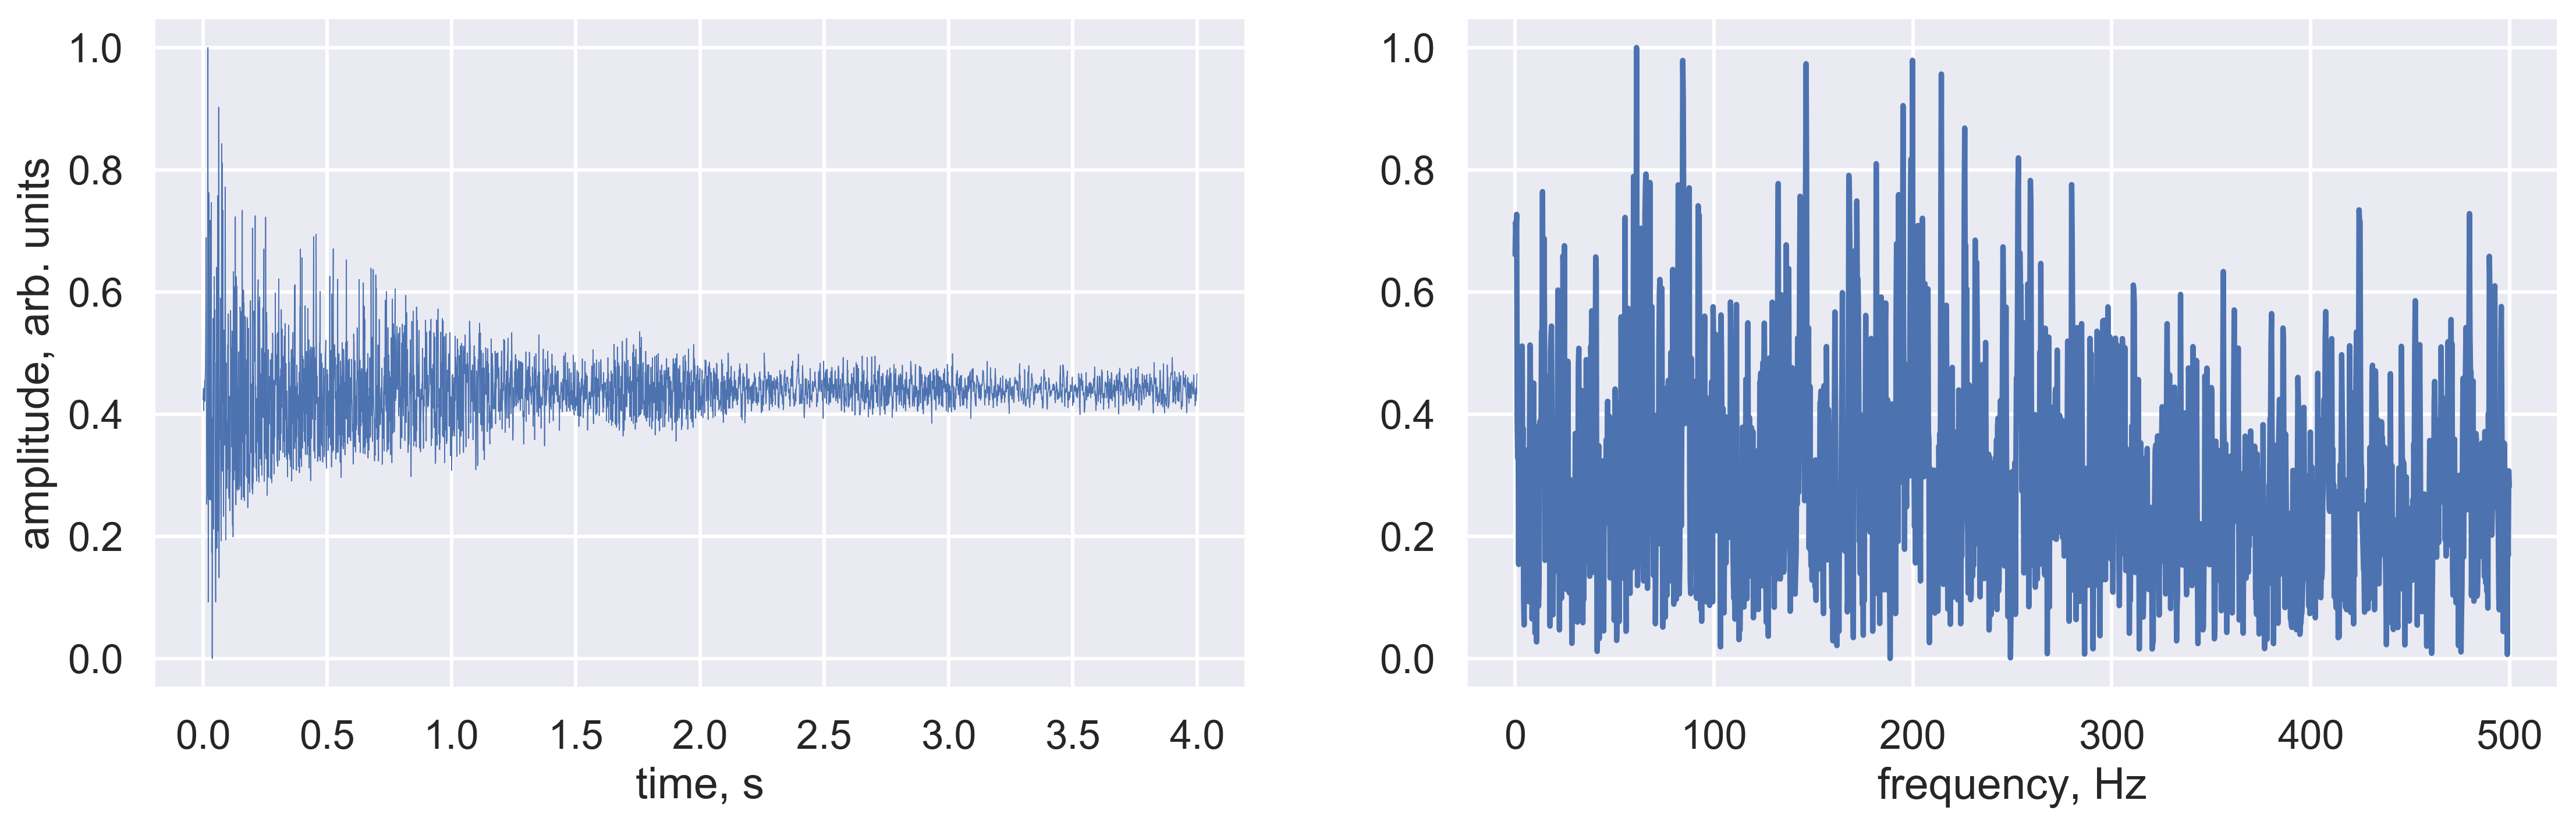
\includegraphics[width=\textwidth]{E1_comp.png}
		\caption{Compressed}
		\label{fig:guitar-compressed}
	\end{subfigure}
	\begin{subfigure}{\textwidth}
		\centering
		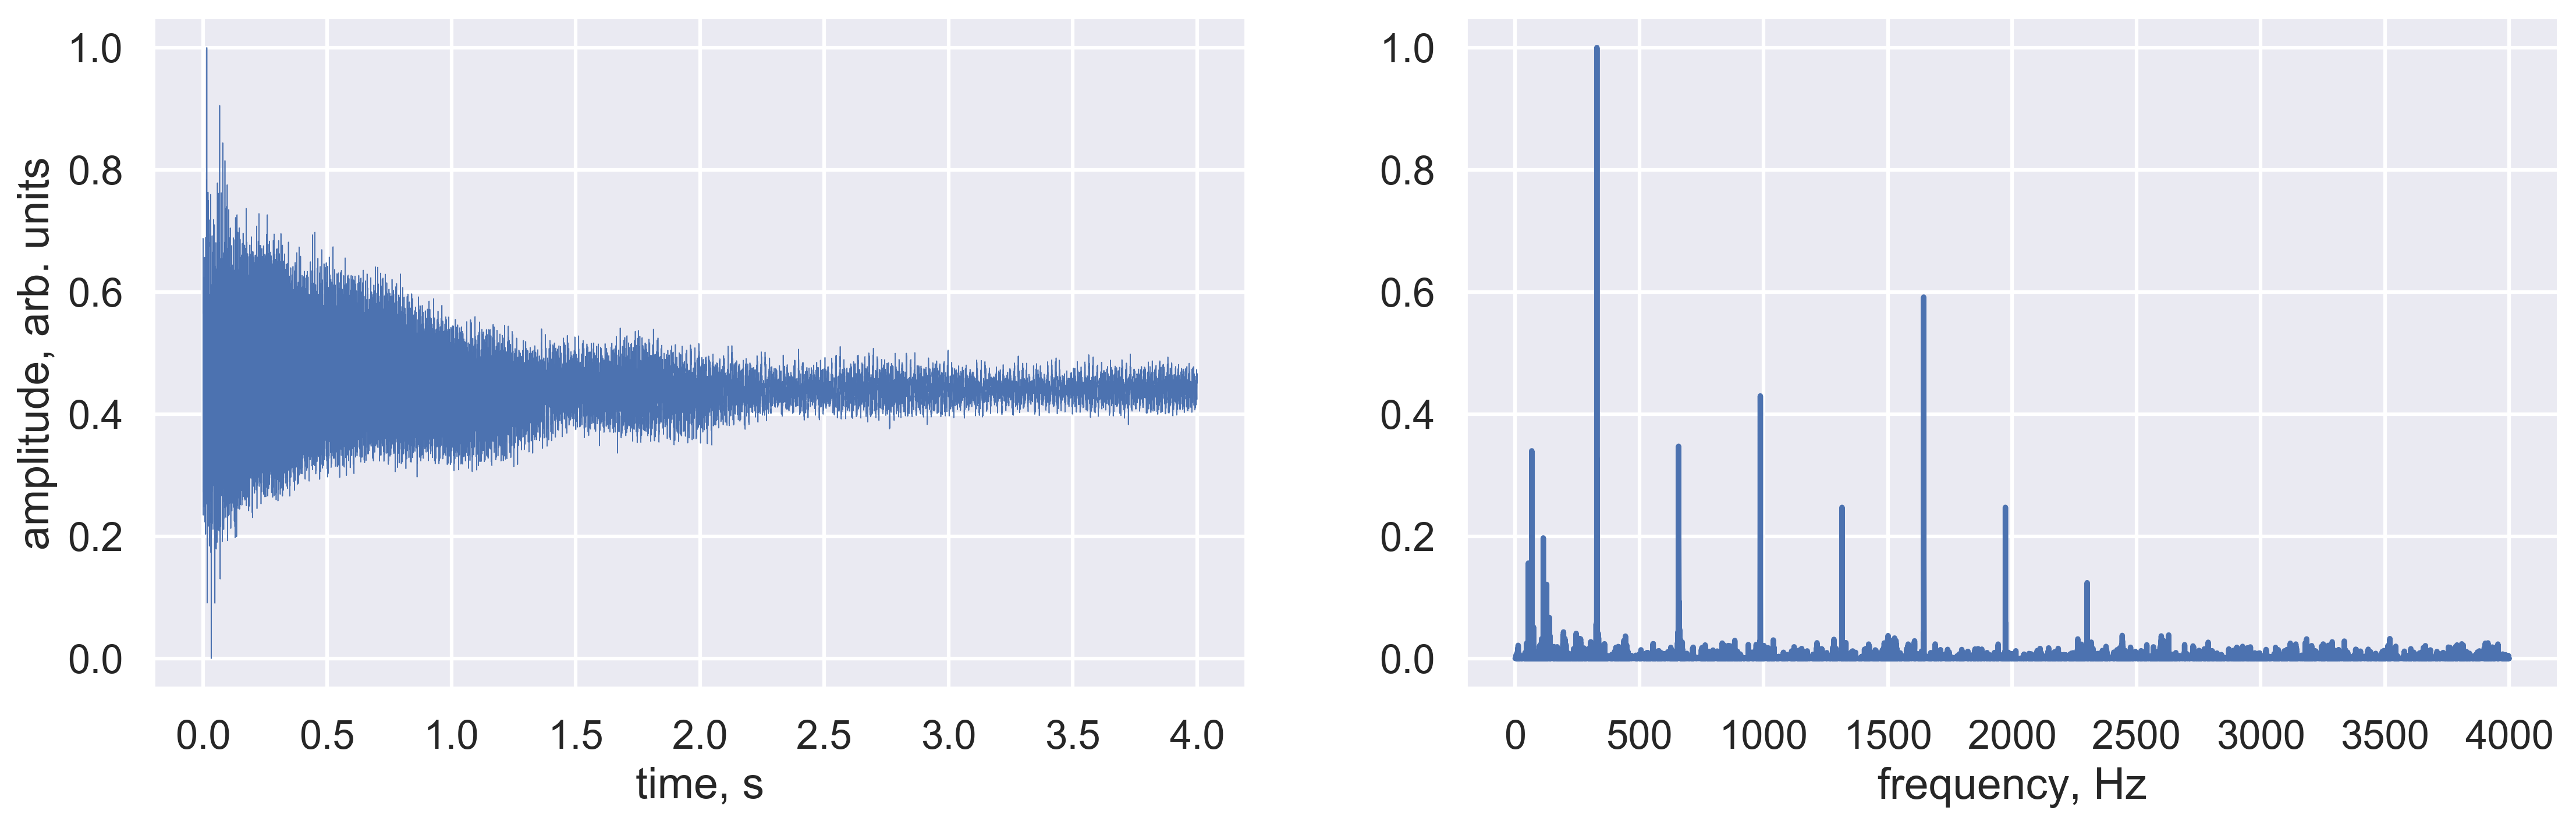
\includegraphics[width=\textwidth]{E1_recov.png}
		\caption{Recovered}
		\label{fig:guitar-recovered}
	\end{subfigure}
	\caption{330 Hz guitar signal representation in the time domain (left column) and frequency domain (right column).}
	\label{fig:guitar}
\end{figure}


\section{Comparison of algorithms}
\label{sec:audio-algorithms}
Following the same procedure as the previous section, my aim now is to compare the performance of three different reconstruction algorithms in terms of average runtime and reconstruction quality. The algorithms used are LASSO and OMP, which were described in Chapter~\ref{chap:theory}. Additionally, the Smoothed L$_0$ Norm (SL0) \cite{Mohimani2009} is used, which approximates the $\ell_0$ norm using a Gaussian of the form

\begin{equation}
	\label{eq:sl0}
	\lim_{\sigma \rightarrow 0} x \exp\qty(-\frac{x^2}{2\sigma^2})
\end{equation}

While all algorithms have polynomial time complexity \cite{Efron2004,Sturm2012,Xiang2019}, OMP shows the worst scaling with respect to time; LASSO and SL0 show similar performance over time (Fig.~\ref{fig:guitar-runtime}). In terms of reconstruction quality (cosine similarity), LASSO is able to breach the 0.8 threshold at 30\% compression ratio, while SL0 achieves this at 50\% compression. On the other hand, OMP shows a nonlinear trend with a large error, which is indicative of unstable performance for low compression ratios (Fig.~\ref{fig:guitar-cossim}).

\begin{figure}[htb]
	\centering
	\begin{subfigure}{0.49\textwidth}
		\centering
		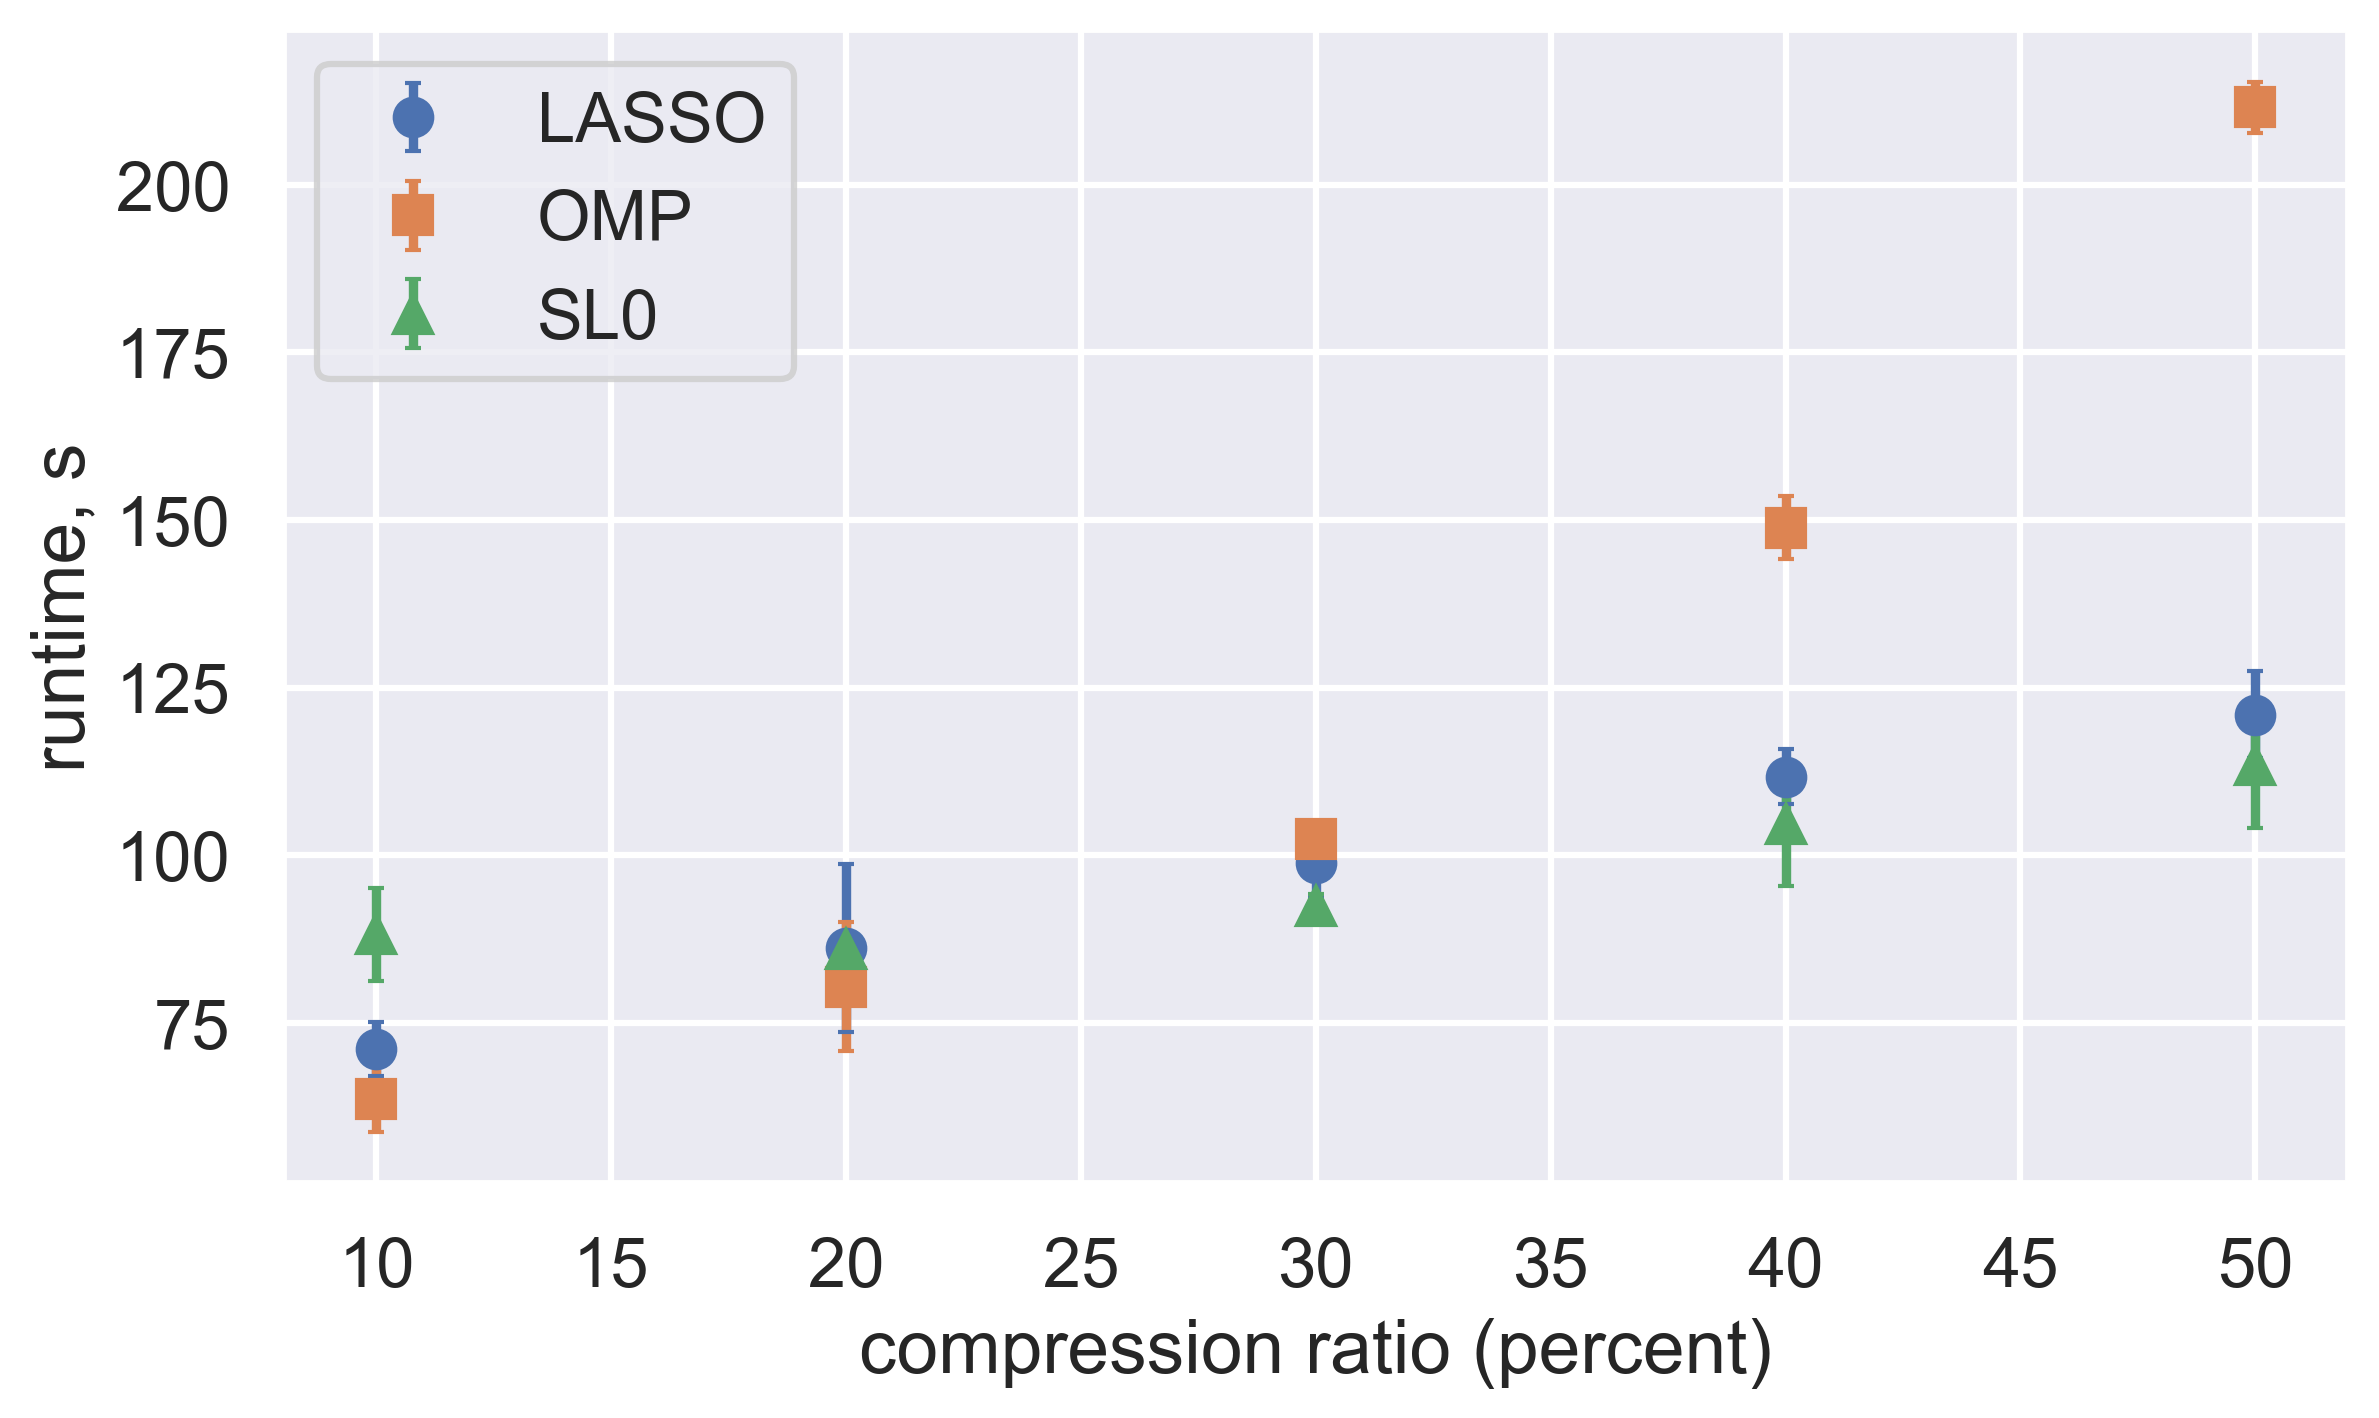
\includegraphics[width=\textwidth]{E1_processtime.png}
		\caption{Runtime}
		\label{fig:guitar-runtime}
	\end{subfigure}
	\begin{subfigure}{0.49\textwidth}
		\centering
		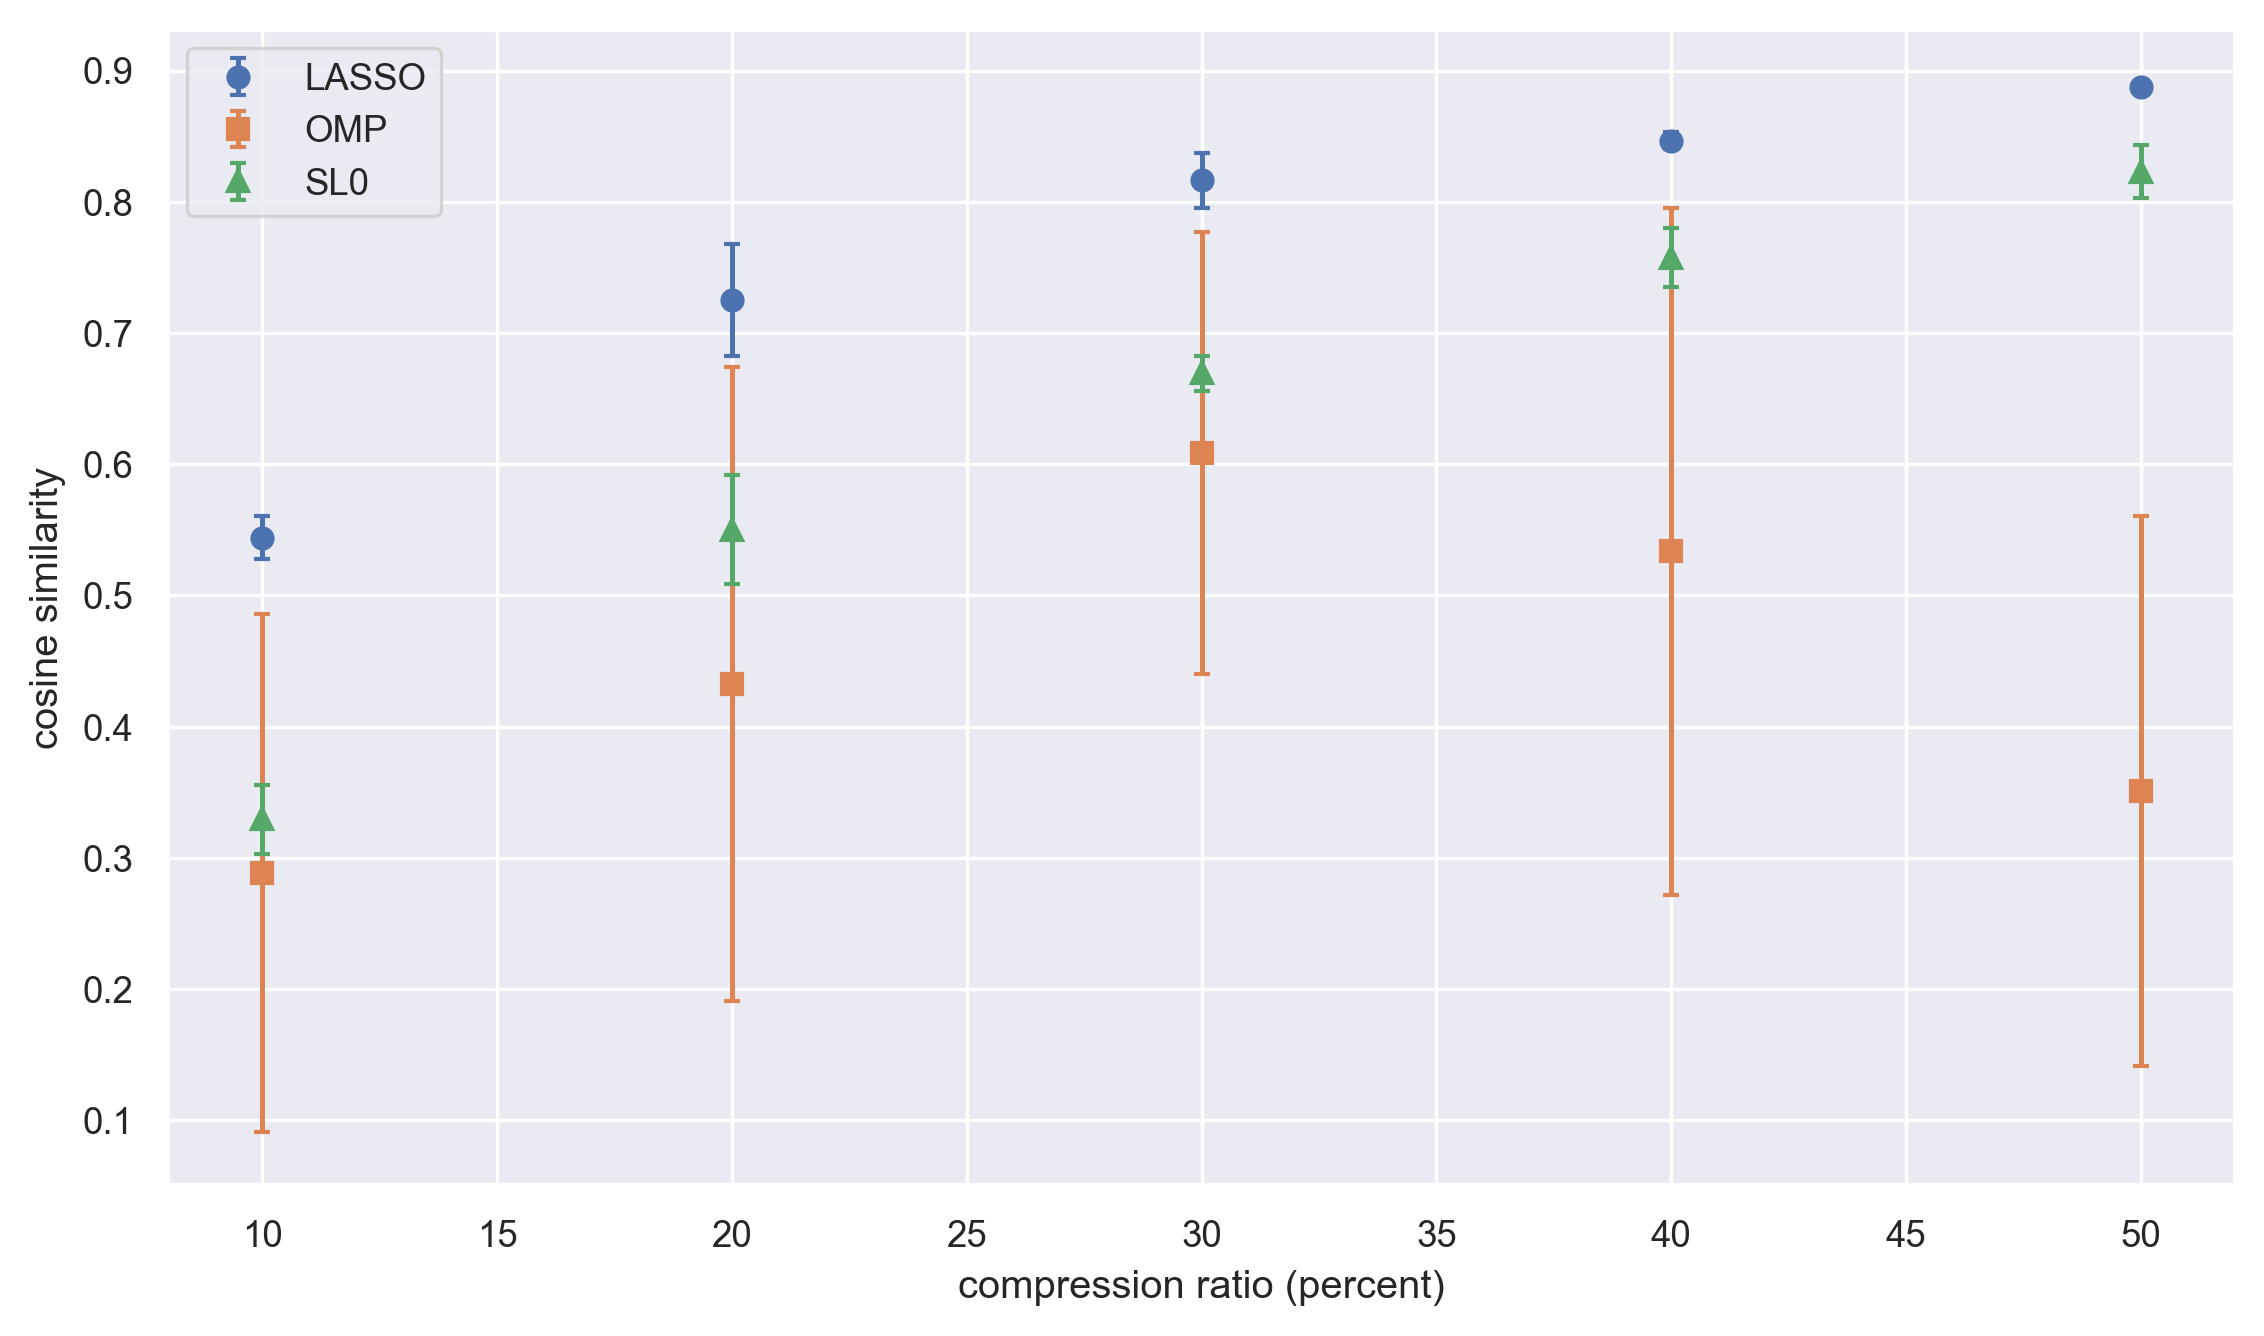
\includegraphics[width=\textwidth]{E1_cossim.png}
		\caption{Reconstruction quality}
		\label{fig:guitar-cossim}
	\end{subfigure}
	\caption{Comparison of the performance of LASSO, OMP, and SL0.}
	\label{fig:guitar-algorithms}
\end{figure}


\section{Speech}
\label{sec:audio-speech}
In order to show its practical merits, we will inevitably have to deal with increasingly large and complex signals. Audio recordings containing speech will encompass a wide range of frequencies, so such signals can only be downsampled so much before essential information is lost to aliasing. Unlike images, large audio signals cannot simply be chopped into smaller, manageable pieces. The effects of aliasing are amplified due to the high information density, and CS' violation of periodic constraints introduce artifacts in the vicinity of where the signal was sliced. This is the motivation for transforming the signal first into the modulation domain (spectrogram).

\subsection{Sparse transformation}
\label{ssec:audio-speech-sparse}
In obtaining the spectrogram representation, first define a short length sampling window, typically only a few milliseconds in duration, as well as the overlap between adjacent frames. The latter is crucial in suppressing boundary artifacts as it ensures that some information from the current measurement is carried over to the next measurement. The signal is then divided into frames by sliding this window across the entire signal. Each frame is multiplied with a window function; in this case, I used the Hann window, defined as

\begin{equation}
	\label{eq:hann-window}
	w[n] = \sin^2\qty(\frac{\pi n}{N})
\end{equation}

\noindent where $N + 1$ is the length of the window, and $n: 0 \leq n \leq N$ is the frame index. Finally, each frame undergoes a Fourier transformation. The entire process is also called a short-time Fourier transform, and is summarized as

\begin{equation}
	\label{eq:stft}
	X(\omega, p) = \sum_{p=0}^{P-1} x[p] w[p - kR] e^{-i\omega p}
\end{equation}

\noindent where $x[p]$ is the $p$th signal frame, $w[p - kR]$ is the window function with hop size $R$ and time index $k$, and $\omega$ is the angular frequency.

\subsection{Pre-processing}
\label{ssec:audio-speech-preprocess}
Test signals were obtained from the TIMIT Acoustic-Phonetic Continuous Speech Corpus \cite{timit}, which contains speech recordings in \texttt{WAV} format. The recordings are of English speakers grouped by region, sex, and unique spoken sentence. All files have a sampling rate of 16 kHz and are, on average, 3 seconds long. I chose a test signal at random, specifically the \texttt{DR8/MJLN0/SA1.wav} file. This indicates that the speaker was from dialect region 8 (nomadic), was male with speaker code \texttt{JLN0}, and spoke unique sentence \texttt{SA1}, which reads

\begin{quotation}
	She had your dark suit in greasy wash water all year.
\end{quotation}

Before proceeding, I downsampled the file to 8 kHz. The representation of the signal in the time and modulation domains are shown in Fig.~\ref{fig:speech-original}.

\begin{figure}[htb]
	\centering
	\begin{subfigure}{0.49\textwidth}
		\centering
		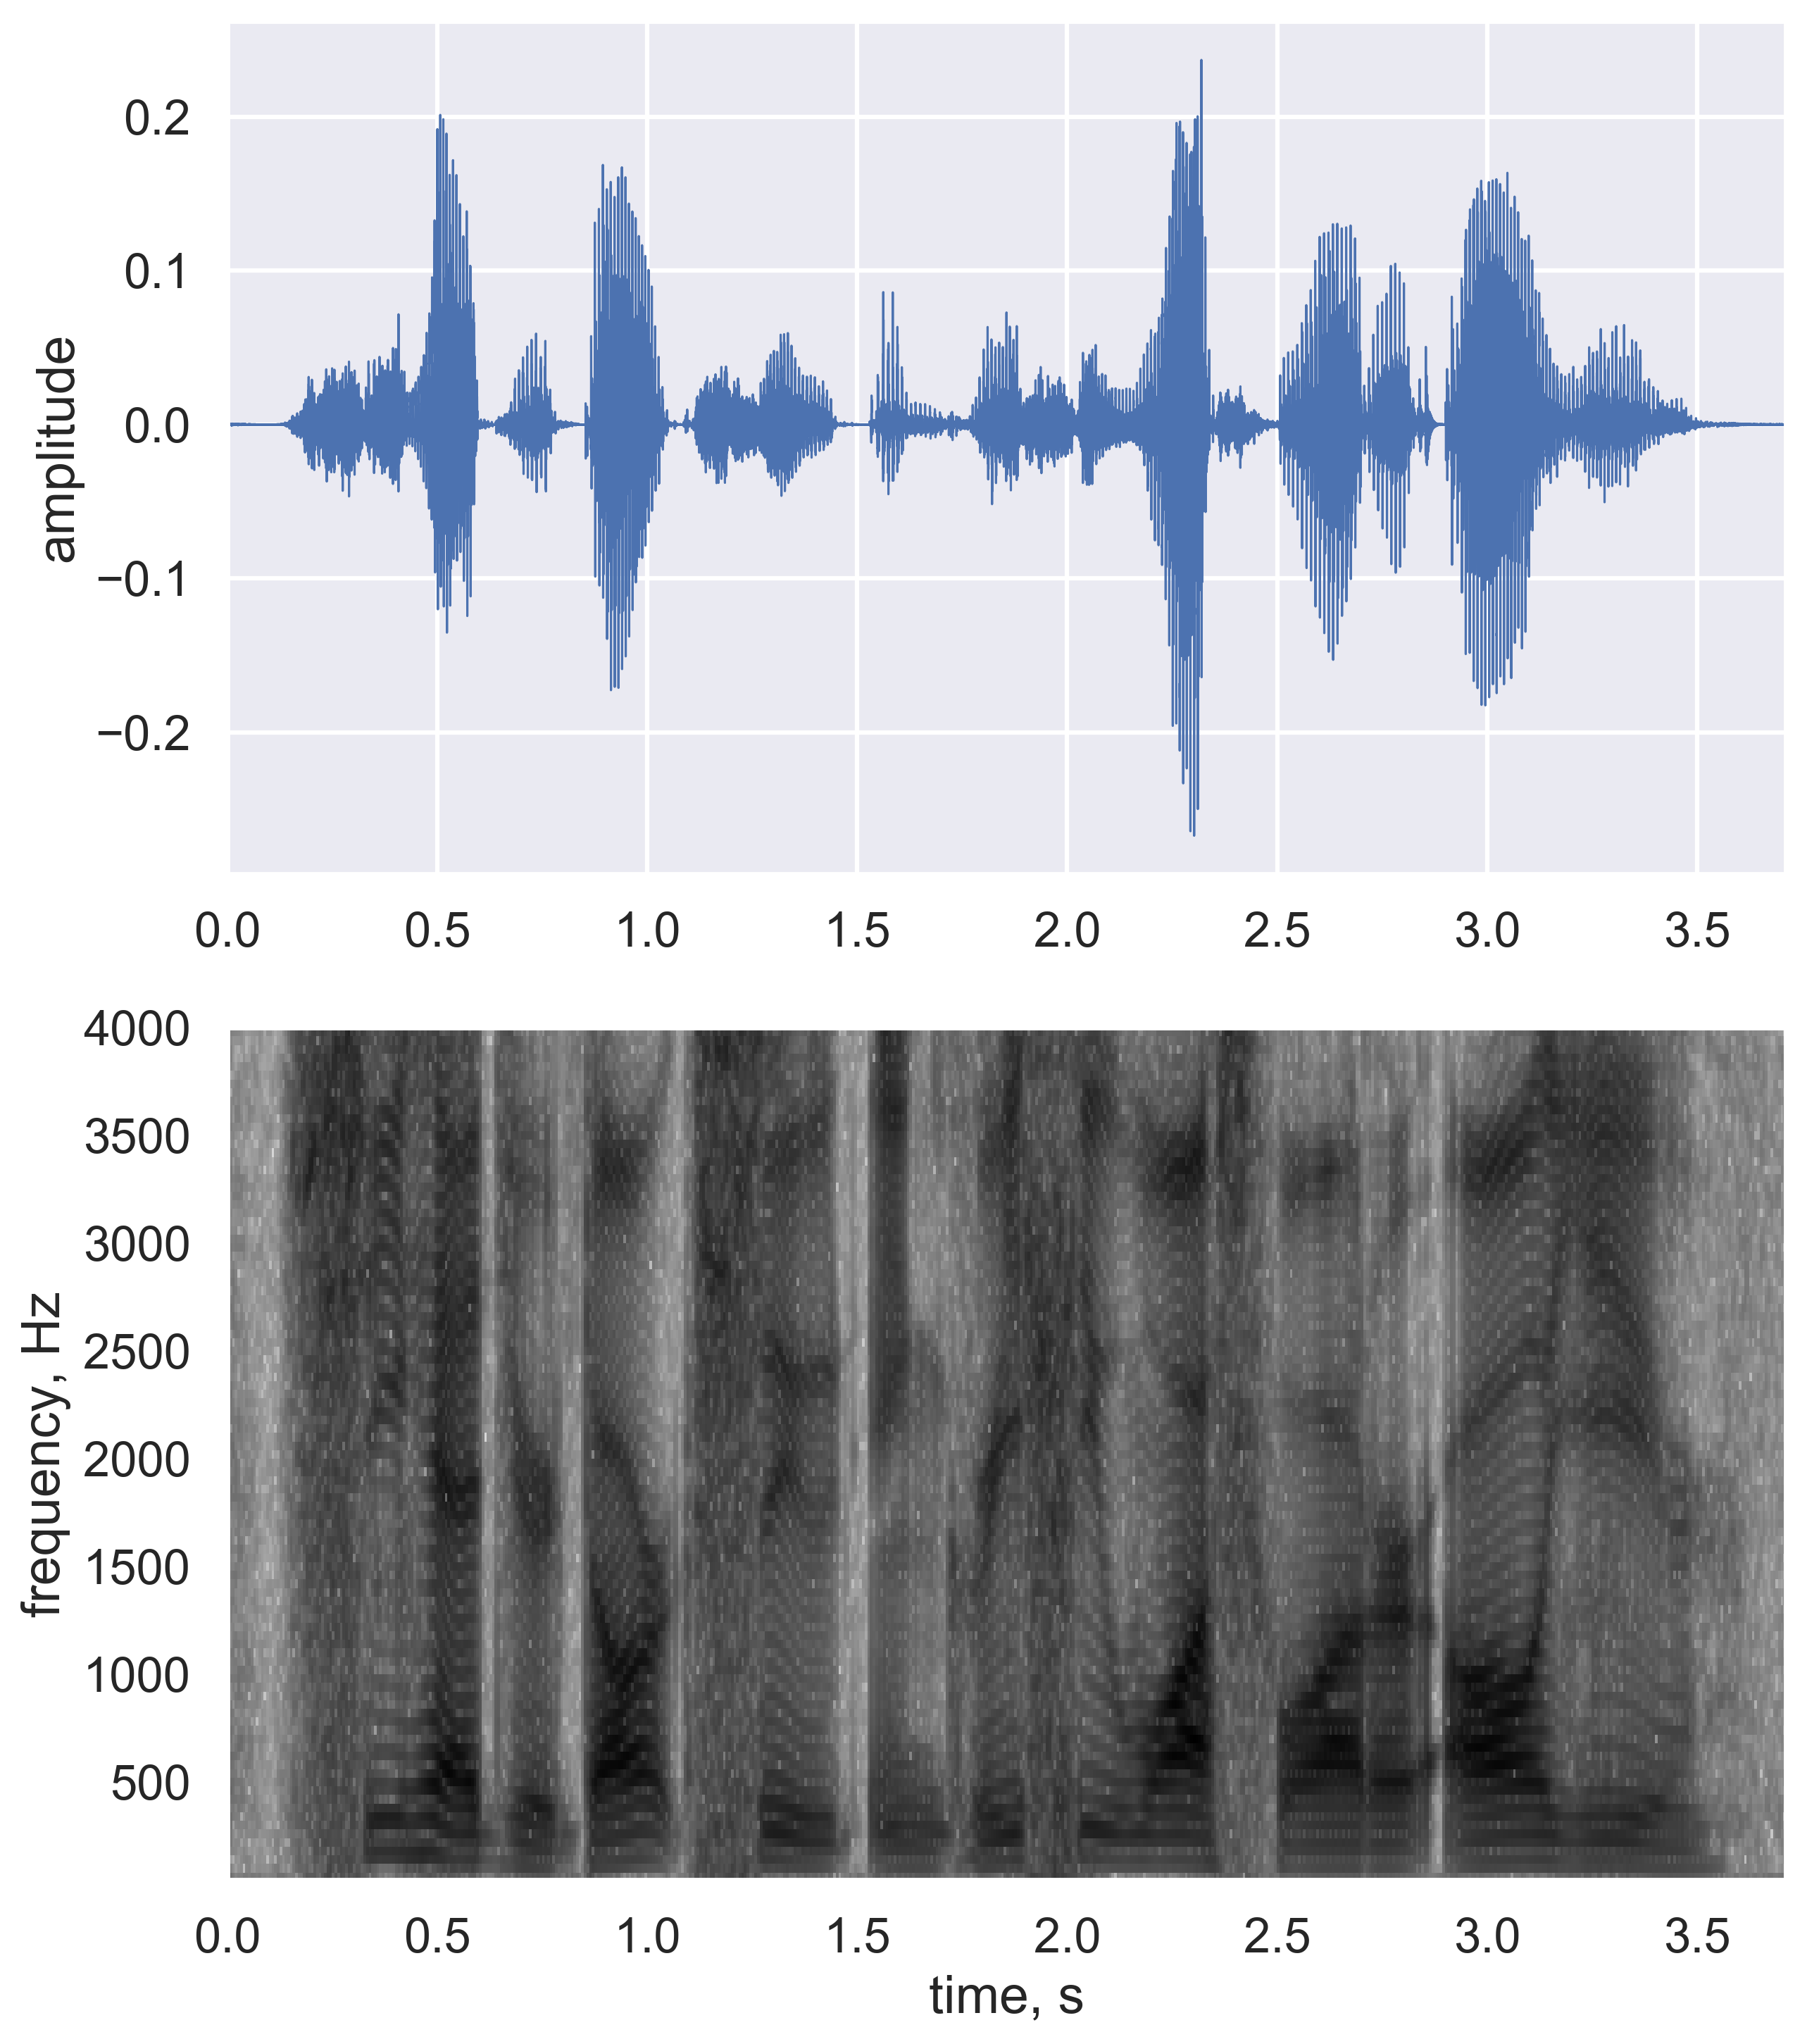
\includegraphics[width=\textwidth]{speech_original.png}
		\caption{Original}
		\label{fig:speech-original}
	\end{subfigure}
	\begin{subfigure}{0.49\textwidth}
		\centering
		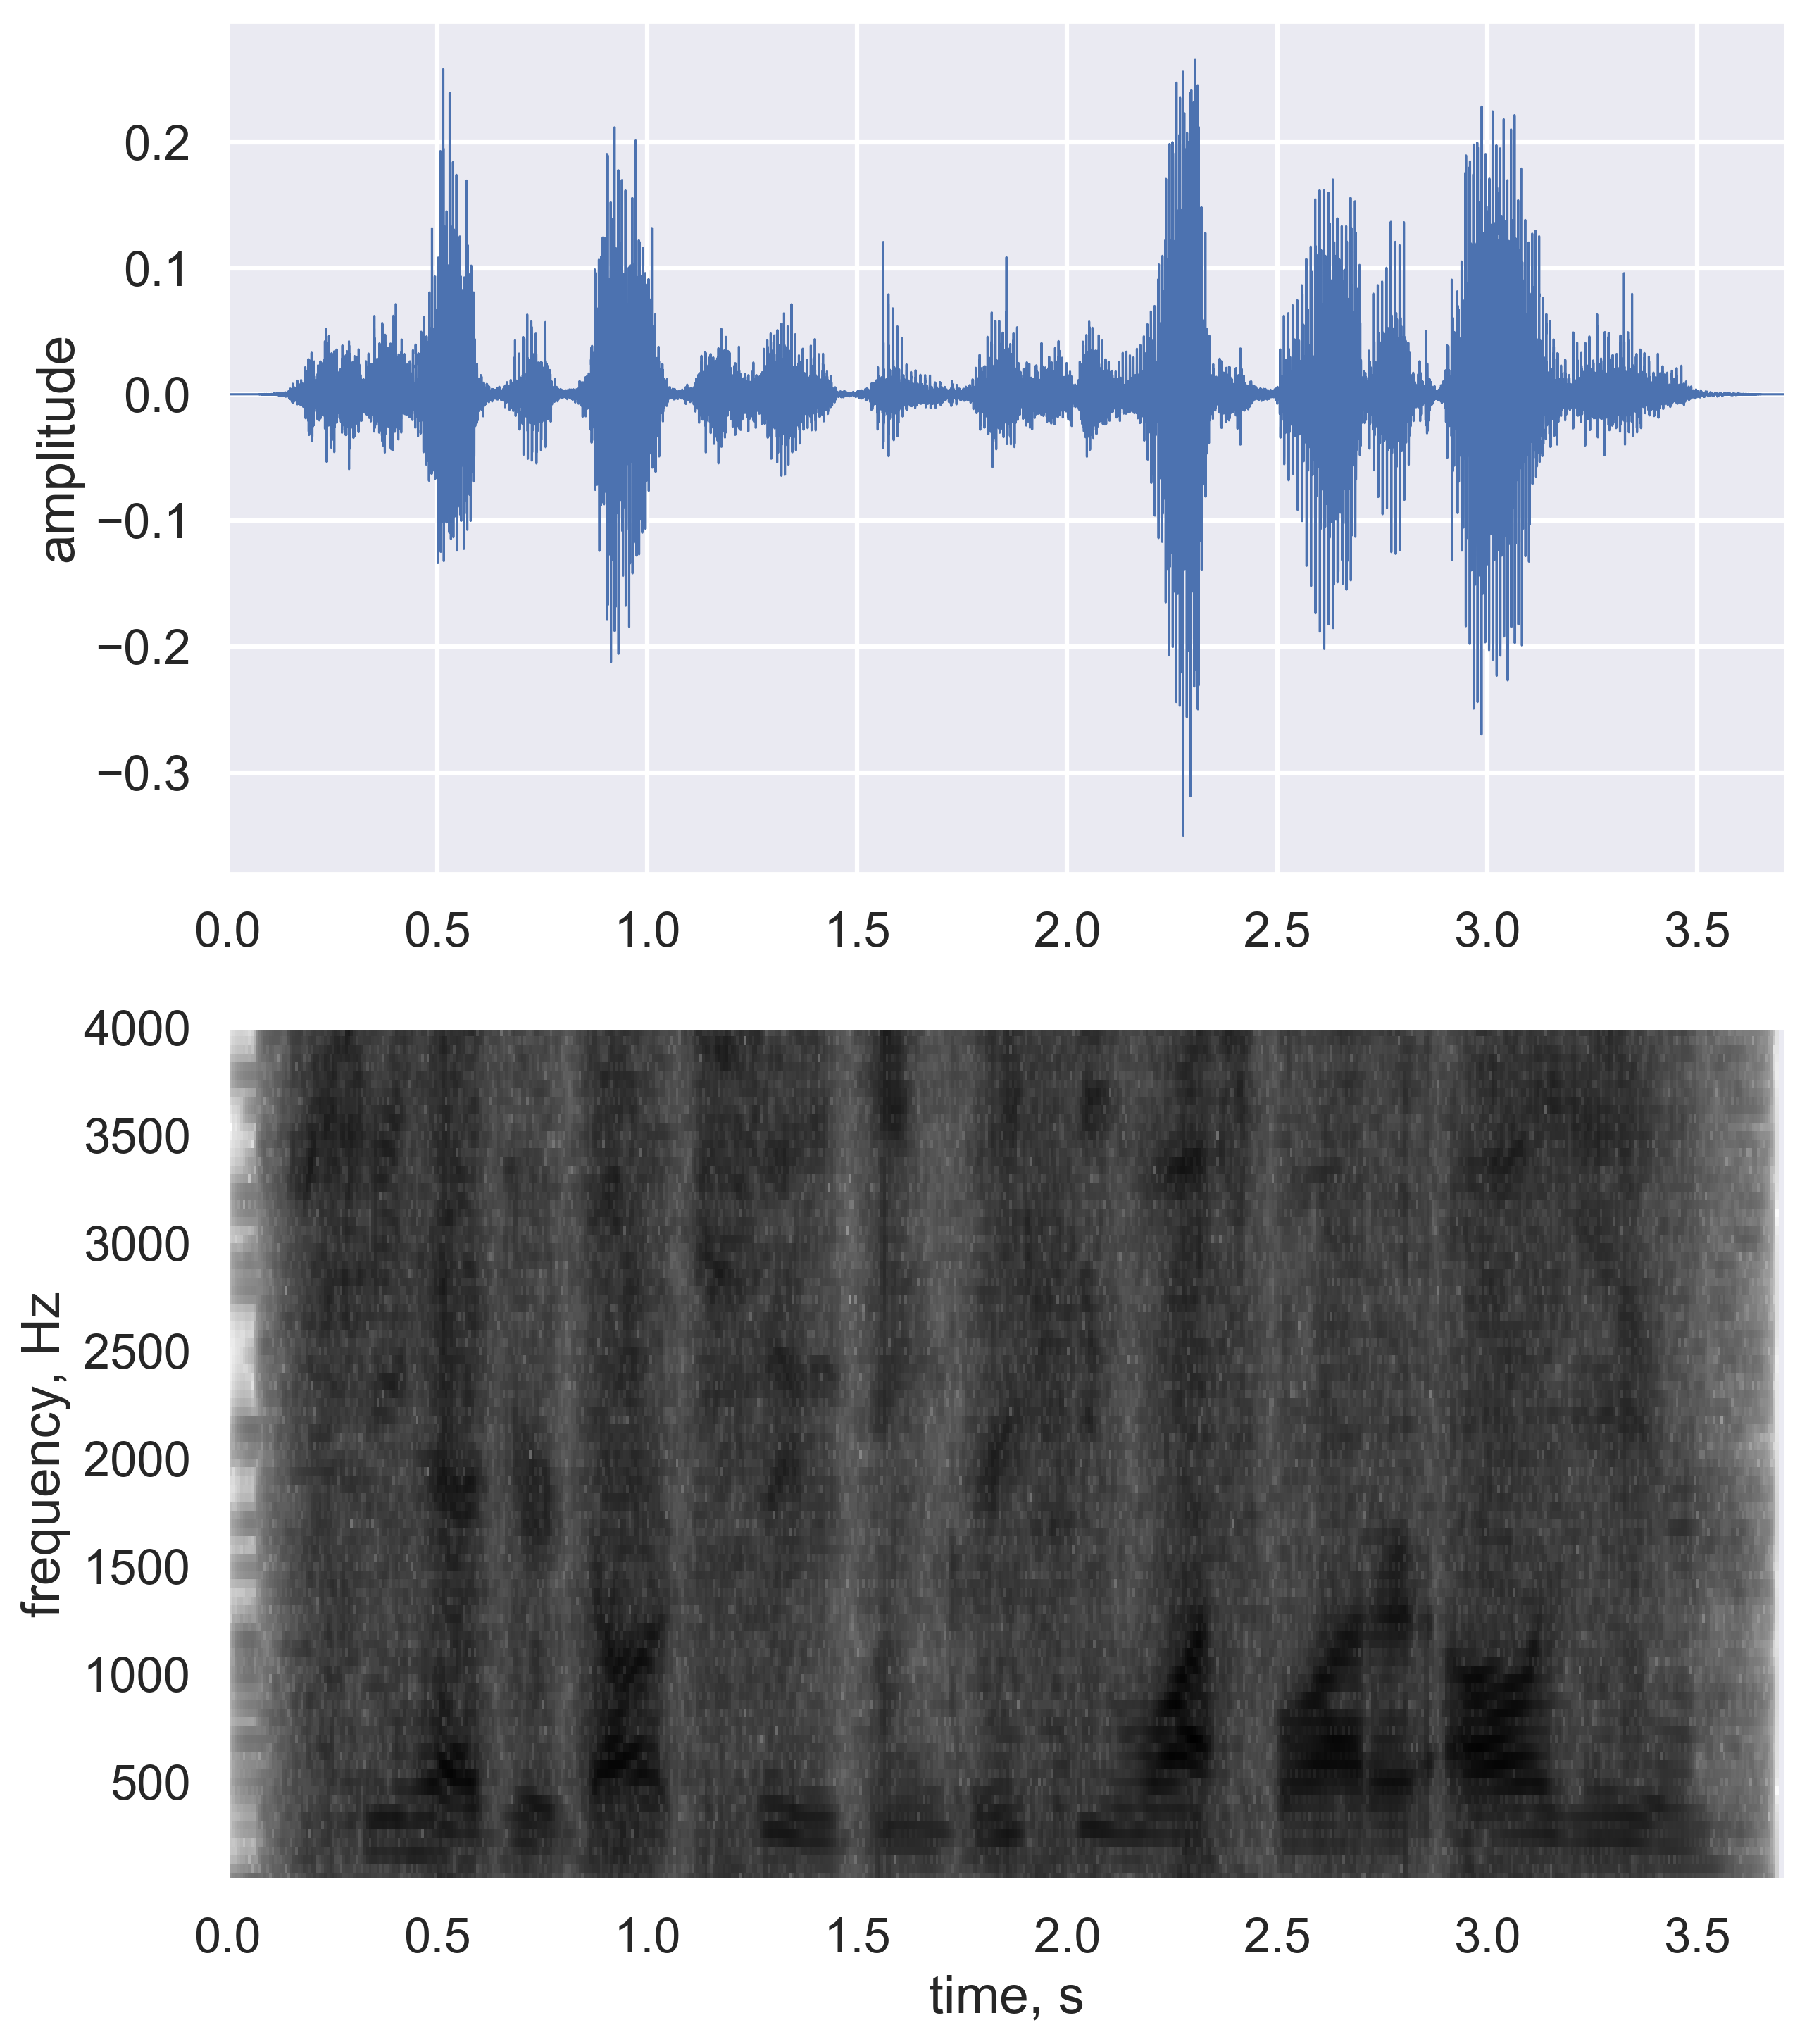
\includegraphics[width=\textwidth]{speech_recover.png}
		\caption{Recovered}
		\label{fig:speech-recovered}
	\end{subfigure}
	\caption{Test speech signal in the time domain (top row) and modulation domain (bottom row).}
	\label{fig:speech}
\end{figure}

\subsection{Processing}
\label{ssec:audio-speech-process}
I compressively sampled the signal with a compression ratio of 40\%, using 1024 frames and 75\% frame overlap. Following the results from Sec.~\ref{sec:audio-algorithms}, I used the LASSO algorithm for reconstruction, once again obtaining the optimal regularization parameter $\alpha$ by 5-fold cross validation.

\subsection{Reconstruction evaluation}
\label{ssec:audio-speech-metric}
The reconstruction quality was quantified using the International Telecommunication Standardization Sector (ITU-T) recommendation P.862 \cite{pesq}, otherwise known as the Perceptual Evaluation of Speech Quality (PESQ). This metric is a full-reference, perceptually intuitive scoring system which models the now-obsolete mean opinion scores (MOS). This algorithm performs a series of standardized tests modeled after qualitative metrics, analyzes and compares the original and reconstructed signals, and returns a value from 1.0 (bad) to 5.0 (perfect). Because real reconstructed signals are rarely exactly the same as the original, the PESQ values are usually thresholded up to 4.5 (excellent). PESQ values of 3.0 and above indicate acceptable quality.

For a more quantitative test, I also used the average segmental signal-to-noise ratio (SNR\textsubscript{seg}) \cite{Loizou2013}, defined as

\begin{equation}
	\label{eq:snrseg}
	\mathrm{SNR_{seg}} = \frac{10}{B} \sum_{b=0}^{B-1} \log_{10} \frac{\sum_{i = Nb}^{Nb + N - 1} x_i^2}{\sum_{i = Nb}^{Nb + N - 1} (x_i - \hat{x}_i)^2}
\end{equation}

\noindent where $N$ is the frame length, $B$ is the number of frames, $x_i$ are the original signal samples, and $\hat{x}_i$ are the reconstructed signal samples.

Figure~\ref{fig:speech-recovered} shows the reconstructed signal. Qualitative comparison in the time domain shows that the original and reconstructed waveforms are structurally similar. In the modulation domain, the dynamic range of the latter seems to have diminished, but the dominant frequencies can still be observed. Evaluation of the PESQ and SNR$_\mathrm{seg}$ yields values of 2.50 and 0.07, respectively. At face value, I can immediately tell from the PESQ that the reconstructed signal quality is slightly below average; listening to the reconstructed recording reveals a noticeable level of noise in the background. However, the same distinction cannot be made for the SNR$_\mathrm{seg}$ since its bounds are not well-defined.

\subsection{Error space analysis}
\label{ssec:audio-speech-error}
Using the same test signal, I generated the error space maps by compressively sampling the signal and evaluating the metrics for varying compression $\textrm{ratios} \in [0.1, 0.9]$ in increments of 0.1, and varying number of $\textrm{frames} \in \{128, 256, 512, 1024\}$, while keeping the frame overlap constant at 75\%. Figure~\ref{fig:speech-error} shows the PESQ and SNR$_\mathrm{seg}$ maps. The former exhibits a sensitivity to the compression ratio, and achieves the acceptable threshold of 3.0 at around 60\% compression. The latter shows sensitivity towards the number of frames (as it is an \textit{average} metric) with some additional degradation below 40\% compression ratio. It achieves a maximum value of 0.08 at around 1024 frames.

\begin{figure}[htb]
	\centering
	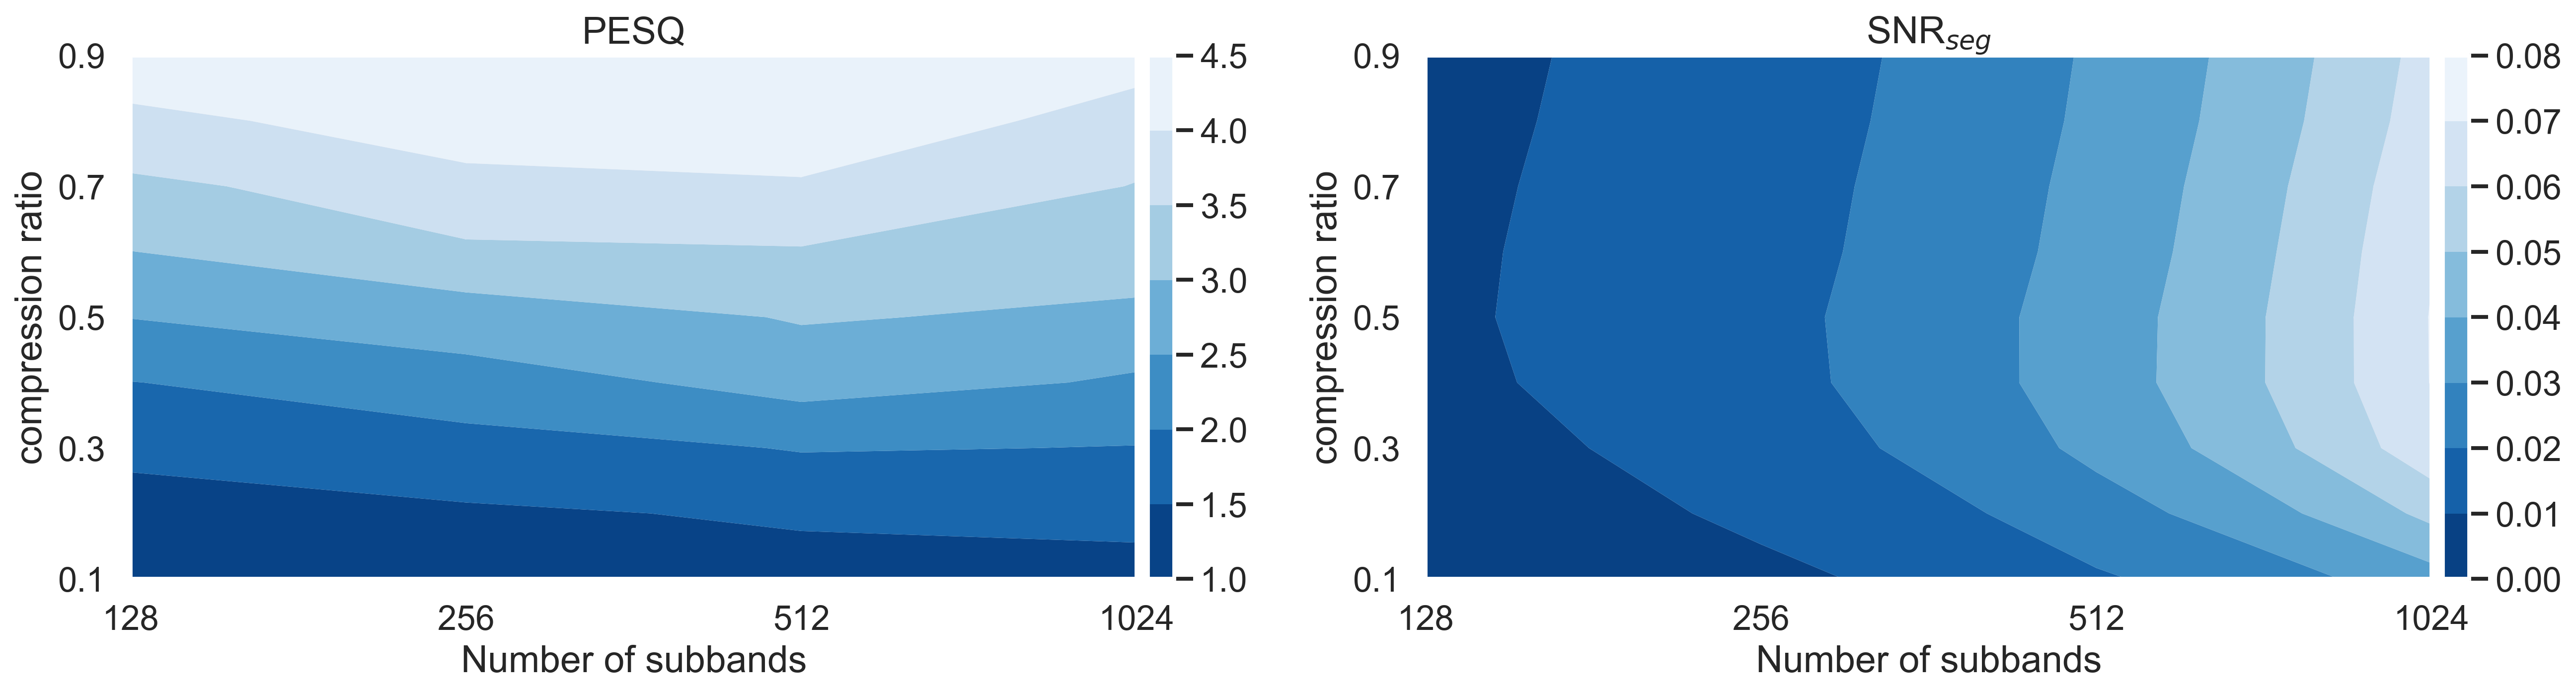
\includegraphics[width=\textwidth]{speech_metrics.png}
	\caption{PESQ and SNR$_\mathrm{seg}$ error space maps as a function of compression ratio and number of subbands.}
	\label{fig:speech-error}
\end{figure}